% -*- root: ../main.tex -*-
%!TEX root = ../main.tex
% this file is called up by main.tex
% content in this file will be fed into the main document
% vim:textwidth=80 fo=cqt

As  evidenced by  the  results of  the constant  current  charge, discharge  and
dynamic  simulation runs,  the basic  \gls{spm} suffers  from a  \emph{critical}
drawback. The lack of electrolyte dynamics in the conventional \gls{spm} results
in poor  voltage accuracy  even at  moderate {C-rates}.  This renders  the model
unsuitable for  observer design in  \gls{soc} estimation applications  since the
output voltage from the model maps  to a radically different \gls{soc} operating
point. A number of candidate solutions have been proposed in literature in order
to mitigate this drawback. Their salient aspects are briefly evaluated here.

Even  the earliest  works which  attempt  to include  electrolyte dynamics  into
the  conventional  \gls{spm} were  published  only  within the  present  decade.
Schmidt~\etal~\cite{Schmidt2010c} proposed  an infinite-sum  eigenfunction modal
expansion paradigm for solving for the electrolyte concentration. It was claimed
that by  accounting for contribution from  only the first two  terms, sufficient
accuracy may be achieved. Furthermore, an \gls{ode} was proposed for the rate of
evolution of  the first temporal  mode. The solved electrolyte  concentration is
then  substituted into  an  approximate analytical  solution  for the  \gls{dfn}
model's  charge conservation  \gls{pde}\fxnote{cross-reference  to newman  model
equation here}  to obtain the  electrolyte potential. However,  the presentation
lacks the  sufficient depth  of explanation  which hinders  reproducibility. For
instance,  the  origin  and  explanation  of  the  approximation  terms  in  the
electrolyte  potential solution  is omitted.  Derivations are  performed from  a
rigorous mathematical perspective without providing contextual reference to cell
parameters or  electrochemical quantities. Introducing numerical  examples would
have been a redeeming factor to help keeping the mathematical aspects tractable.
This method has not seen further uptake for \gls{spm} modelling.

Guo~\etal~\cite{Guo2011}  presented   an  empirical  approach  to   account  for
the  solution-phase   dynamics.  Using  standard  curve-fitting   techniques,  a
non-linear   resistance  as   a  function   of  current   and  temperature   was
introduced.   Thus,   the  equation   for   cell   terminal  voltage   presented
in~\cref{eq:cellterminalvoltagebasic} is modified as
\begin{equation}
    V_\text{cell} = η_\text{pos} - η_\text{neg} + U_\text{pos} - U_\text{neg} - I R_\text{eq}
\end{equation}
where  $R_\text{eq}$  is the  equivalent  resistance  newly introduced.  In  the
opinion of  this thesis  author, this  approach is too  simplistic and  does not
generalise well. Even if giving up  physics-based model origins can be tolerated
for one  or two subsystems  within the model,  the equivalent resistance  is not
just a minor correction term since it  needs to account for a large polarization
voltage of  the order  of tens of  millivolts. Secondly,  the current-dependence
introduced  to account  for the  complex mass  and charge  transport within  the
electrolyte  places a  disproportionately large  weight on  the accuracy  of the
curve-fitting process. Non-linear fits as proposed in Guo~\etal{} are inherently
problematic  in nature  as  the optimisation  routine may  converge  to a  local
minimum.  The specific  form and  nature, \eg{}  the convexity  of the  proposed
hypothesis function is  not discussed. Also, it is also  not guaranteed that the
same fitting  function is  applicable to  a different cell  with another  set of
parameters. Finally,  the correction  term being resistive  in nature  is zeroth
order,  \ie{}  cannot account  for  the  frequency  dependent behaviour  of  the
electrolyte's  dynamics. This  approach is  more suited  for small-scale  static
corrections that do not depend on the current,\eg{} to account for a few tens of
microvolts  due to  a constant  contact  resistance of  the current  collectors.
\fxnote{later on, as a capstone work, mention how I was inspired}

Di   Domenico~\etal{}~\cite{DiDomenico2010}  were   the  first   to  present   a
step-by-step  derivation   of  the   approximate  analytical  solution   to  the
electrolyte overpotential. The potential drop in the electrolyte is given by
\begin{equation}\label{eq:electrolytepd}
    \phi_\epos - \phi_\eneg = -\frac{I}{2 A}\left(\frac{l_\text{neg}}{\kappa_\text{eff}} + 2 \frac{l_\text{sep}}{\kappa_\text{eff}} + \frac{l_\text{pos}}{\kappa_\text{eff}}\right)
\end{equation}
and     can     be     substituted    into     the     subtraction     operation
involving~\cref{eq:posoverpotential} and~\cref{eq:negoverpotential} in computing
the   overall  overpotential   of~\cref{eq:overpotentialdifference}  and   hence
the  terminal  voltage.  The  effective   conductivity  of  the  electrolyte  in
a   given   region   \jinpossepneg{},   within   the   cell,   is   defined   as
$\kappa_\effj(c_e) = \kappa(c_e)\, \varepsilon_j^{\text{brugg}_j}$. As discussed
in~\cref{subsec:basicspmsimsetup},  the   intrinsic  and  hence   the  effective
electrolyte conductivity is a function of the concentration of \ch{Li^+} ions in
the  electrolyte.  Di  Domenico~\etal{}  did  not  discuss  the  spatio-temporal
calculation  of  electrolyte  concentration.  It   is  likely  that  a  constant
electrolyte concentration  at its  initial equilibrium value  was used.  As seen
in~\cref{fig:ce1cdischgwithzoom}\fxnote{do not  forget to  show the  gradient in
$c_e$}, significant spatial gradients in the electrolyte are established at even
low to moderate {C-rates} during  the cell's operation. Sustained application of
a unidirectional  current even leads to  starvation of ions in  the electrolyte,
particularly  near  the  current   collectors.  This  phenomenon  is  visualised
in~\cref{fig:ce1cdischgwithzoom} wherein the electrolyte at the positive current
collector  is  virtually  depleted  of  ions  at  the  end  of  discharge.  This
ion-starvation process occurs earlier at higher {C-rates} and spreads throughout
the thickness of the electrode.  Furthermore, Di Domenico~\etal{} do not present
any results of  applying dynamic current profiles. Since the  critical aspect of
mass transport contribution to electrolyte  overpotential is omitted, this model
cannot be viewed as a \emph{sufficient} enhancement to the basic \gls{spm}.

\begin{figure}[!htp]
    \centering
    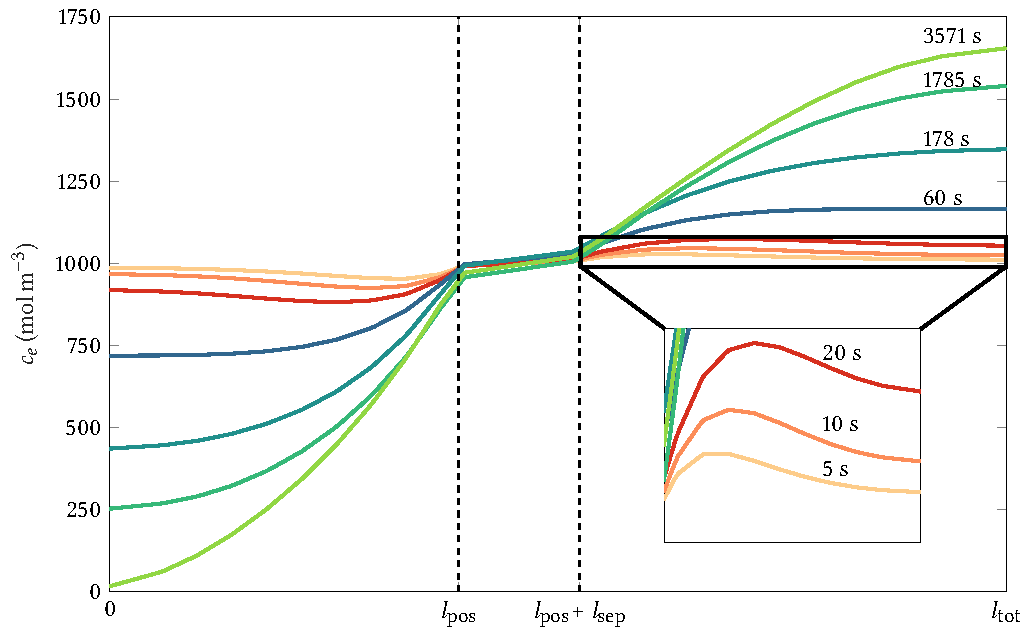
\includegraphics{4/figures/ce_1C_at_various_times.pdf}
    \caption[Electrolyte conc.\ (time-snapshots) along cell thickness for 1C
    discharge]{Spatial distribution of \ch{Li^+} ion concentration in
        electrolyte along cell thickness at various time-snapshots during a 1C
        discharge lasting \SI{3571}{\second}. A \glsfmtlong{qss}
        (\glsfmtshort{qss}) spatial profile  with inflection point at each
        separator interface begins to form at \approx \SI{60}{\second} after
        discharge begins. However, the ionic concentration in electrolyte
        exhibits a significantly different transient behaviour (zoomed inset)
        possessing another inflection point that disrupts the monotonic trend.
        Depletion of ionic concentration at positive current collector  towards
    end of discharge is shown.}
    \label{fig:ce1cdischgwithzoom}
\end{figure}

Although  not presented  in the  context  of incorporating  into the  \gls{spm},
Guduru~\etal~\cite{Guduru2012}   derived   an   analytical   solution   of   the
spatio-temporal  evolution  of  electrolyte concentration  using  the  \gls{sov}
method. The \gls{sov} method was first  applied to lithium ion cell modelling by
Subramanian~\etal~\cite{Subramanian2001a}  in order  to  solve  for solid  phase
concentration  profiles in  spherical  electrode particles.  Although the  ionic
concentration  in  the electrolyte  computed  by  the analytical  expression  in
Guduru~\etal{} seems like a feasible choice for inclusion into the \gls{spm}, it
is only applicable for galvanostatic boundary conditions, \ie{} when the applied
current  is held  constant over  time. By  natural extension,  researchers could
hypothesise  that this  restriction  may  be removed  by  considering the  input
current as  piecewise constant  over small sample  intervals. Such  a hypothesis
could  be reinforced  by the  fact that  standard drivecycles  are specified  as
discrete  samples  and  the  discrete-time  \gls{spm}  loops  over  these  input
samples assuming \gls{zoh} behaviour. However, the analytical solution presented
in  Guduru~\etal{}  assumes  a  \gls{qss} concentration  profile.  The  authors'
presentation  considers a  near-instantaneous  establishment  of this  \gls{qss}
and  suggests a  parameter  independent analysis  through  use of  dimensionless
concentrations  and time-constants  instead of  absolute time.

In  the studies  conducted  by this  thesis author,  the  transient duration  of
establishing the  \gls{qss} is not negligible  and exhibits a dependence  on the
parameter set used. \Cref{fig:ce1cdischgwithzoom} shows the spartial

Thus, in  a highly dynamic operating  conditions with frequent reversals  in the
direct of current, the galvanostatic  assumption for analytical solution becomes
harder to uphold without introducing significant errors. Finally, the analytical
solution  to  the concentration  profile  itself  is  not entirely  amenable  to
embedded implementation, since it consists of a non-trivial set of trigonometric
computations at each time-step.


Rahimian~\etal{}~\cite{KhaleghiRahimian2013} discuss  the usage of  a polynomial
approximation  for   electrolyte  concentration  and  potentials.   However,  no
restriction was imposed on the order  of the polynomials chosen to represent the
electrolyte concentration within  each porous electrode region.  In the standard
\gls{dfn} model, the  number of equations and  corresponding boundary conditions
describing electrolyte charge and mass transport within the cell is insufficient
to uniquely solve for all  unknown coefficients of the polynomial approximation.
The  challenges  posed  due  to  this equation  deficiency  shall  be  discussed
in~\cref{temp:eqndeficiency}. Although  the original  \gls{spm} did  not involve
solving  for  the  electrolyte  concentrations  or  potentials,  The  polynomial
approximation of the single


Rahimian~\etal{} adopted  a cubic  polynomial for approximating  the electrolyte
concentration within  the porous electrodes.  To overcome the issue  of equation
deficiency, they adapted a scheme wherein one additional spatial location in the
interior  of  each  electrode  was  used. The  coefficients  of  the  polynomial
approximation  were then  obtained  by iteratively  solving  a relatively  large
coupled  system of  algebraic equations,  embedding within  them the  additional
equations evaluated at  the interior point. An additional  complicating issue is
the specific positioning of this  additional interior point. An online numerical
optimisation  was performed  to obtain  the optimal  placement of  this interior
node. Although it serves as a proof of concept towards implementing higher order
polynomial approximations,  the author of this  thesis deems this method  as too
complex for online implementations.


% A common  characteristic of  these proposals  is that  they seek  to incorporate
% electrolyte  dynamics  of  varying  degrees  of  complexity  directly  into  the
% \gls{spm}. But I did something different.  The high accuracy of the \gls{soc} in
% the basic  \gls{spm} leads to  the author's  hypothesis that if  the electrolyte
% concentration  can  be  solved  as an  independent  subsystem  and  incorporated
% into  the  terminal  voltage,  this  can lead  to  an  improved  \gls{spm}  with
% electrolyte  dynamics. Such  a decoupled  electrolyte inclusion  into the  basic
% \gls{spm}\fxnote{fix this sentence}

